
\documentclass[12pt,a4paper]{cibb}


\usepackage{tikz}
\usepackage{float}
\usetikzlibrary{arrows.meta, positioning}

\usepackage{graphicx}
\usepackage{amsmath,amsfonts,latexsym,amssymb,euscript,xr}
\usepackage{booktabs}
\usepackage{hyperref}


\usepackage{color,colortbl,tabularx}

\usepackage[english]{babel}
\usepackage[protrusion=true,expansion=true]{microtype}
\usepackage{amsmath,amsfonts,amsthm}
% \usepackage[pdftex]{graphicx}
\usepackage{pifont}

\def\red{\color{red}}
\def\black{\color{black}}
\def\blue{\color{blue}}
\def\magenta{\color{magenta}}

\definecolor{LightBlue}{rgb}{0.88,0.9,0.9}




\title{\Large $\ $\\ \bf Data Analytics AI Powered Spreadsheet}

\author{\large Vijay Balaji$^1$, Vivswan Savyasachi$^{2}$, and Reeshabh Kotecha$^{3}$}
\address{\footnotesize $\ $\\$^1$ 2023CS51103 \\
%
$^2$ 2023CS10699 \\
%
$^3$ 2023CS10018 \\
%

}


\abstract{\normalsize
\\[17pt]
{\bf Abstract.} In this document we explain our design decisions for implementing the Rust Lab and our extension.}

\begin{document}
\thispagestyle{myheadings}
\pagestyle{myheadings}
\markright{\tt COP290 Rust Lab}%check year



\section{\bf Introduction}


As part of our spreadsheet extension, we implemented a frontend web interface that communicates seamlessly with a backend server responsible for data persistence and processing. When a user modifies a cell in the frontend, a POST request is sent to the backend. The server processes the update and returns a list of affected cells along with their updated values, ensuring consistency across dependent cells.

On the frontend, we introduced several data analytics features to enhance user comprehension and engagement. These tools enable users to easily visualize trends and extract insights from the data.

Additionally, we integrated an AI-assisted formula generation feature. This component leverages a large language model (LLM) to suggest the next formula based on the last five user-defined formulas. 

\section{Backend Architecture Overview}

The backend is organized into two primary modules: \texttt{input} and \texttt{spreadsheet}. These are supported by a foundational \texttt{basic} module, which defines common \texttt{structs} and \texttt{enums} shared across the system. A \texttt{main} module orchestrates the interaction between these components, adapting to the specific use case.

\subsection*{\texttt{basic} Module}
Contains shared data structures and definitions used across both \texttt{input} and \texttt{spreadsheet}, promoting code reuse and modularity. It contains the Formula struct and Expression enum, which contain the different types of possible input expressions.

\begin{verbatim}
pub struct Formula {
    pub inp_cell: Cell,
    pub expression: Expression,
}
\end{verbatim}

\subsection*{\texttt{input} Module}
Responsible for parsing and validating user inputs. The following public function takes any argument implementing the BufRead trait as input and outputs a Formula Option. The get formula function is called in the main function of the spreadsheet. 

\begin{verbatim}
pub fn get_formula<R: BufRead>(reader: &mut R) -> Option<Formula>
\end{verbatim}

The following two functions are used by the spreadsheet module to convert column numbers to letter format for printing purposes.

\begin{verbatim}
pub fn from_num(mut num: u32) -> Option<Col>
pub fn as_str(&self) -> &str
\end{verbatim}

\begin{figure}[H]
    \centering
    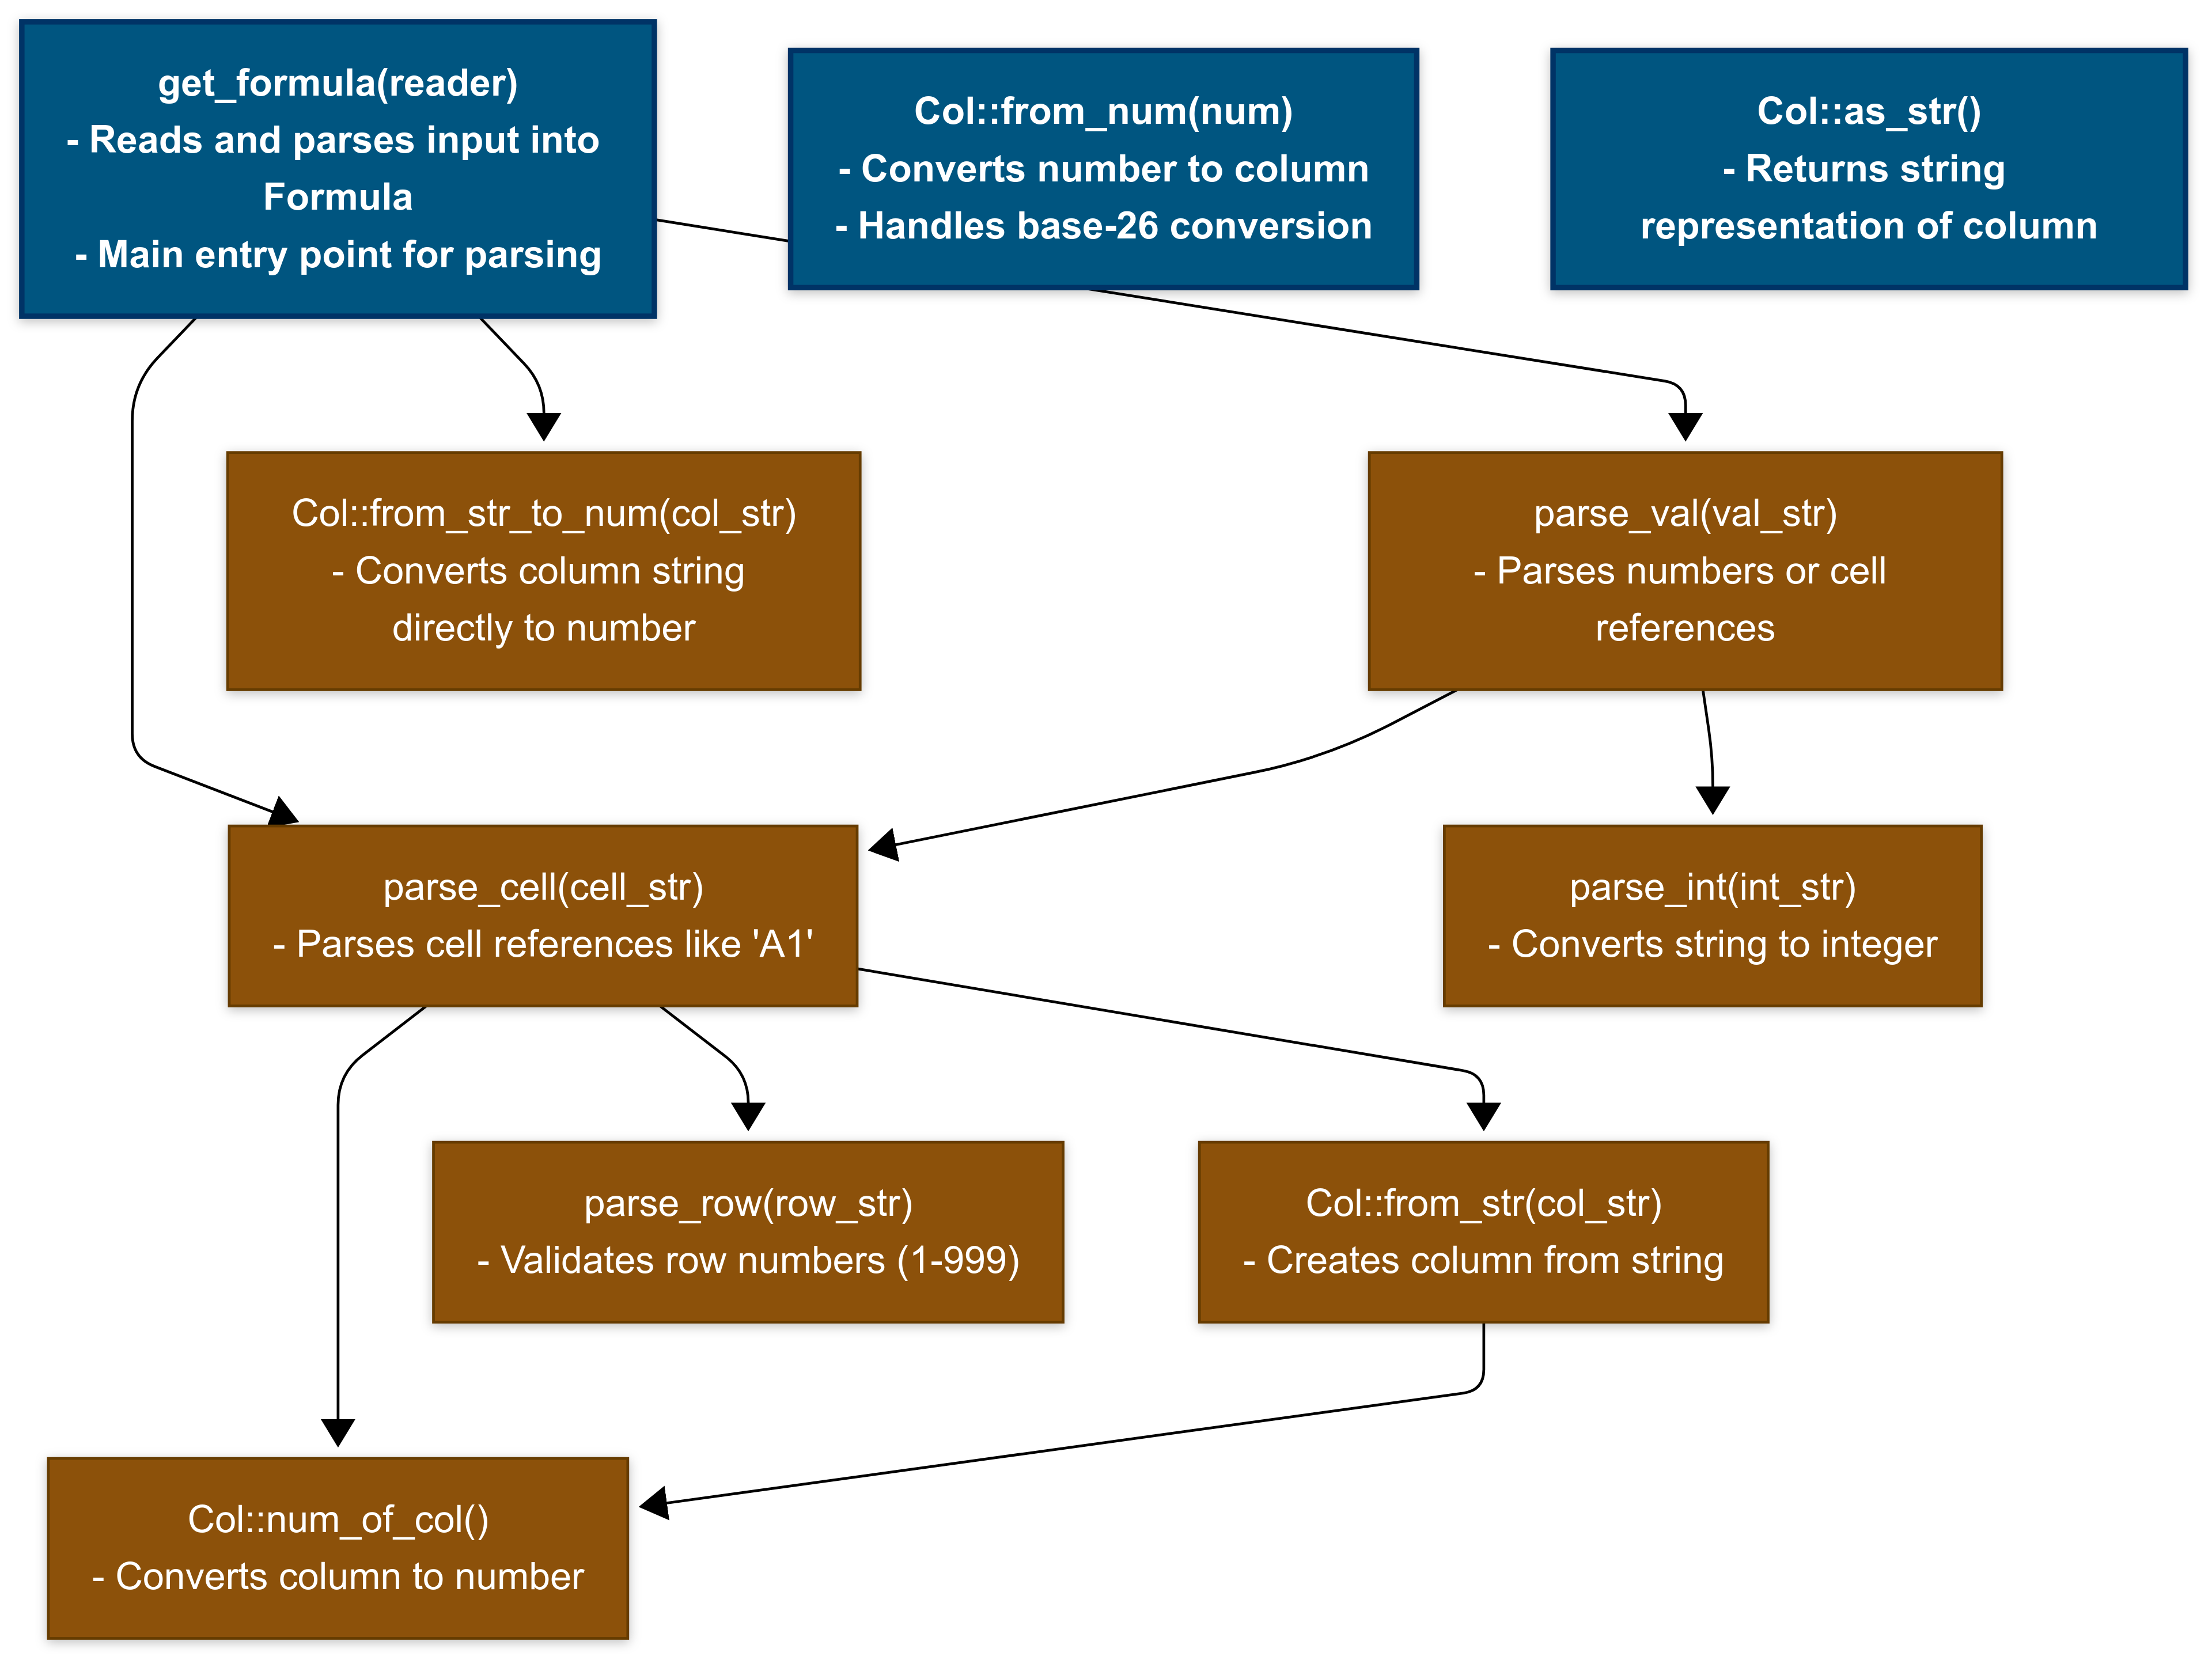
\includegraphics[width=0.75\linewidth]{input_module.png}
    \caption{Input Module}
    \label{fig6}
\end{figure}

\subsection*{\texttt{spreadsheet} Module}
Handles the core spreadsheet logic, including cell evaluation, dependency tracking, and formula computation.

The main function will start by initializing the spreadsheet with the given number of rows and cols using the public function new. Once the spreadsheet has been created, the only way to interact with the sheet is by adding a new formula, or querying the contents of the sheet by printing.

\begin{verbatim}
pub fn new(row: usize, col: usize) -> SpreadSheet
pub fn call_formula(&mut self, form: Option<Formula>) -> SpreadSheetError
pub fn print_sheet(&self)
\end{verbatim}

\begin{figure}[H]
    \centering
    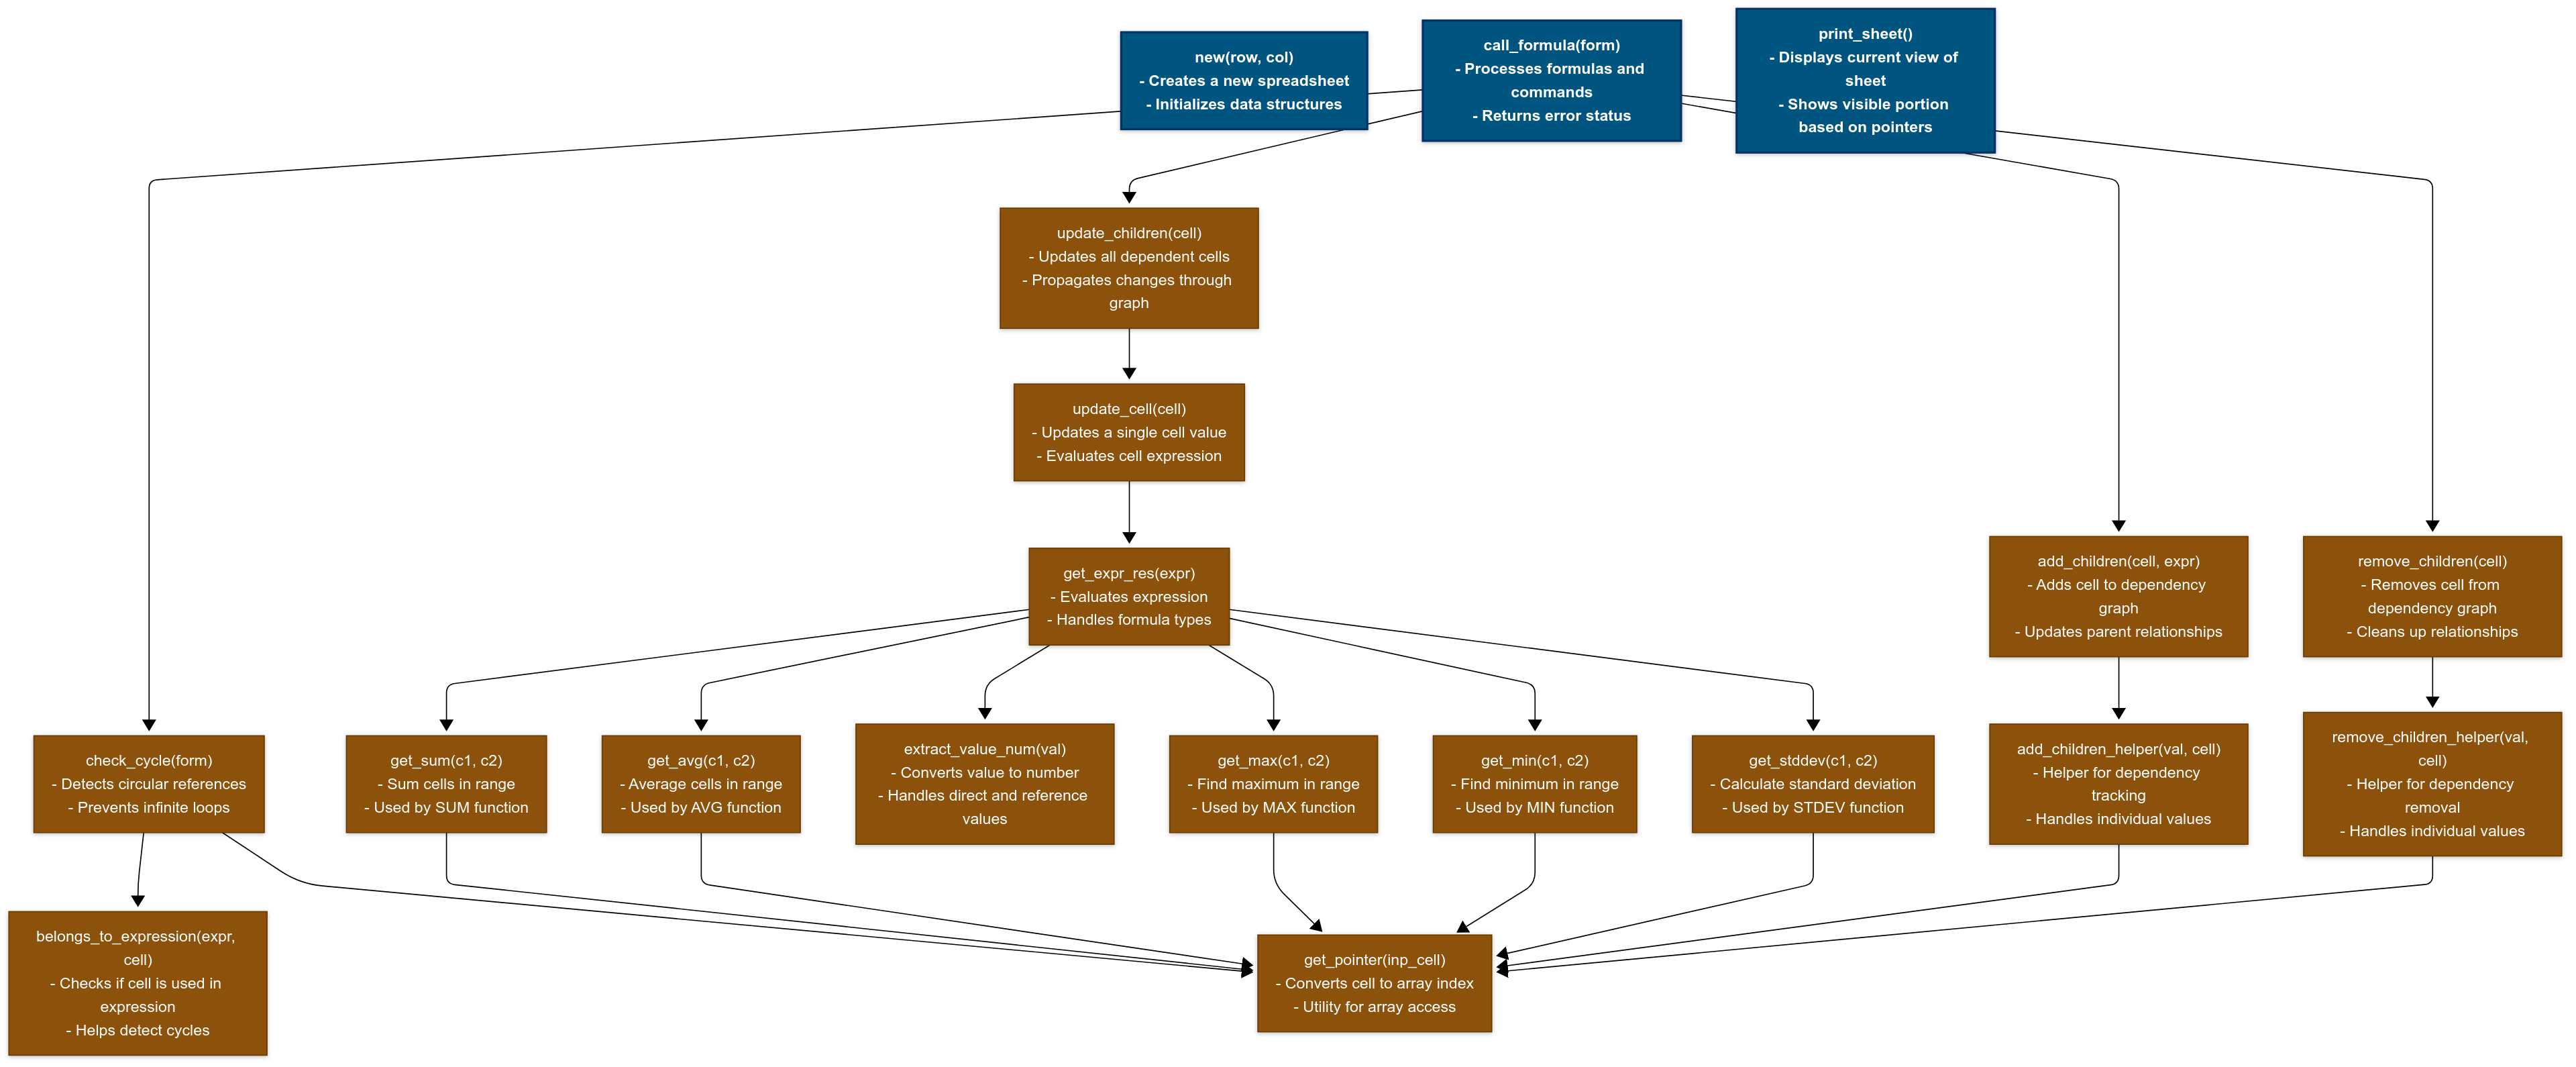
\includegraphics[width=1\linewidth]{spreadsheet_module.png}
    \caption{SpreadSheet Module}
    \label{fig7}
\end{figure}

We use a spreadsheet struct to house the primary data structures for the spreadsheets and for a class like implementation in a programming language like rust that does not support objects.

\begin{verbatim}
pub struct SpreadSheet {
    row_pointer: usize,
    col_pointer: usize,
    row: usize,
    col: usize,
    spreadsheet: Vec<CellData>,
    val: Vec<i32>,
    valid: Vec<u8>,
    exprs: HashMap<Cell, Expression>,
    constant_mode: u32,
}
\end{verbatim}


\begin{itemize}
    \item \textbf{val Vector:} Stores individual cell values in a single contiguous block of memory. This design maximizes cache efficiency, especially for range operations.
    
    \item \textbf{valid Flags:} Maintained in a contiguous memory block. If the \texttt{valid} flag is set to 1 for a cell, it indicates that the cell is invalid and an \texttt{err} is displayed (e.g., due to division by zero or dependency on another \texttt{err} cell).
    
    \item \textbf{Expression HashMap:} Since most cells are initialized with constant integers, using an expression field for every cell is memory-inefficient. Therefore, expressions are stored only for relevant cells in a \texttt{HashMap}.
    
    \item \textbf{Children Set (CellData):} Stores dependent children cells using a \texttt{HashSet}. Like \texttt{val} and \texttt{valid}, this is stored in a contiguous memory block for performance.
    
    \item \textbf{row and col Pointers:} \texttt{row\_pointer} and \texttt{col\_pointer} mark the current cursor location used by the \texttt{print} method.
    
    \item \textbf{row and col Sizes:} \texttt{row} and \texttt{col} store the dimensions of the spreadsheet.
    
    \item \textbf{Constant Mode Flag:} Used to determine whether a formula is constant and thus can skip cycle checks or complex computation. For instance, a formula that evaluates to a single integer does not require further processing.
\end{itemize}

For the backend version of the spreadsheet module, we have made slight modifications. The call formula function will also return a list of cells and their modified values in the form of a string so that it can be parsed into a json and be returned to the Post request.


\subsection*{\texttt{main} Module}
Acts as the integration layer. In the terminal-based interface, it manages I/O with the user via the terminal. In the server-based configuration, it handles HTTP(S) requests and responses, serving as the entry point for web clients.

We have the POST method, get value, which takes a json containing the input cell and expression. It applies this formula to the spreadsheet and returns the changed cells and their values.

\begin{verbatim}
async fn get_value(
    State(state): State<AppState>,
    Json(params): Json<CellParams>,
) -> Json<serde_json::Value>
\end{verbatim}

\begin{figure}[H]
    \centering
    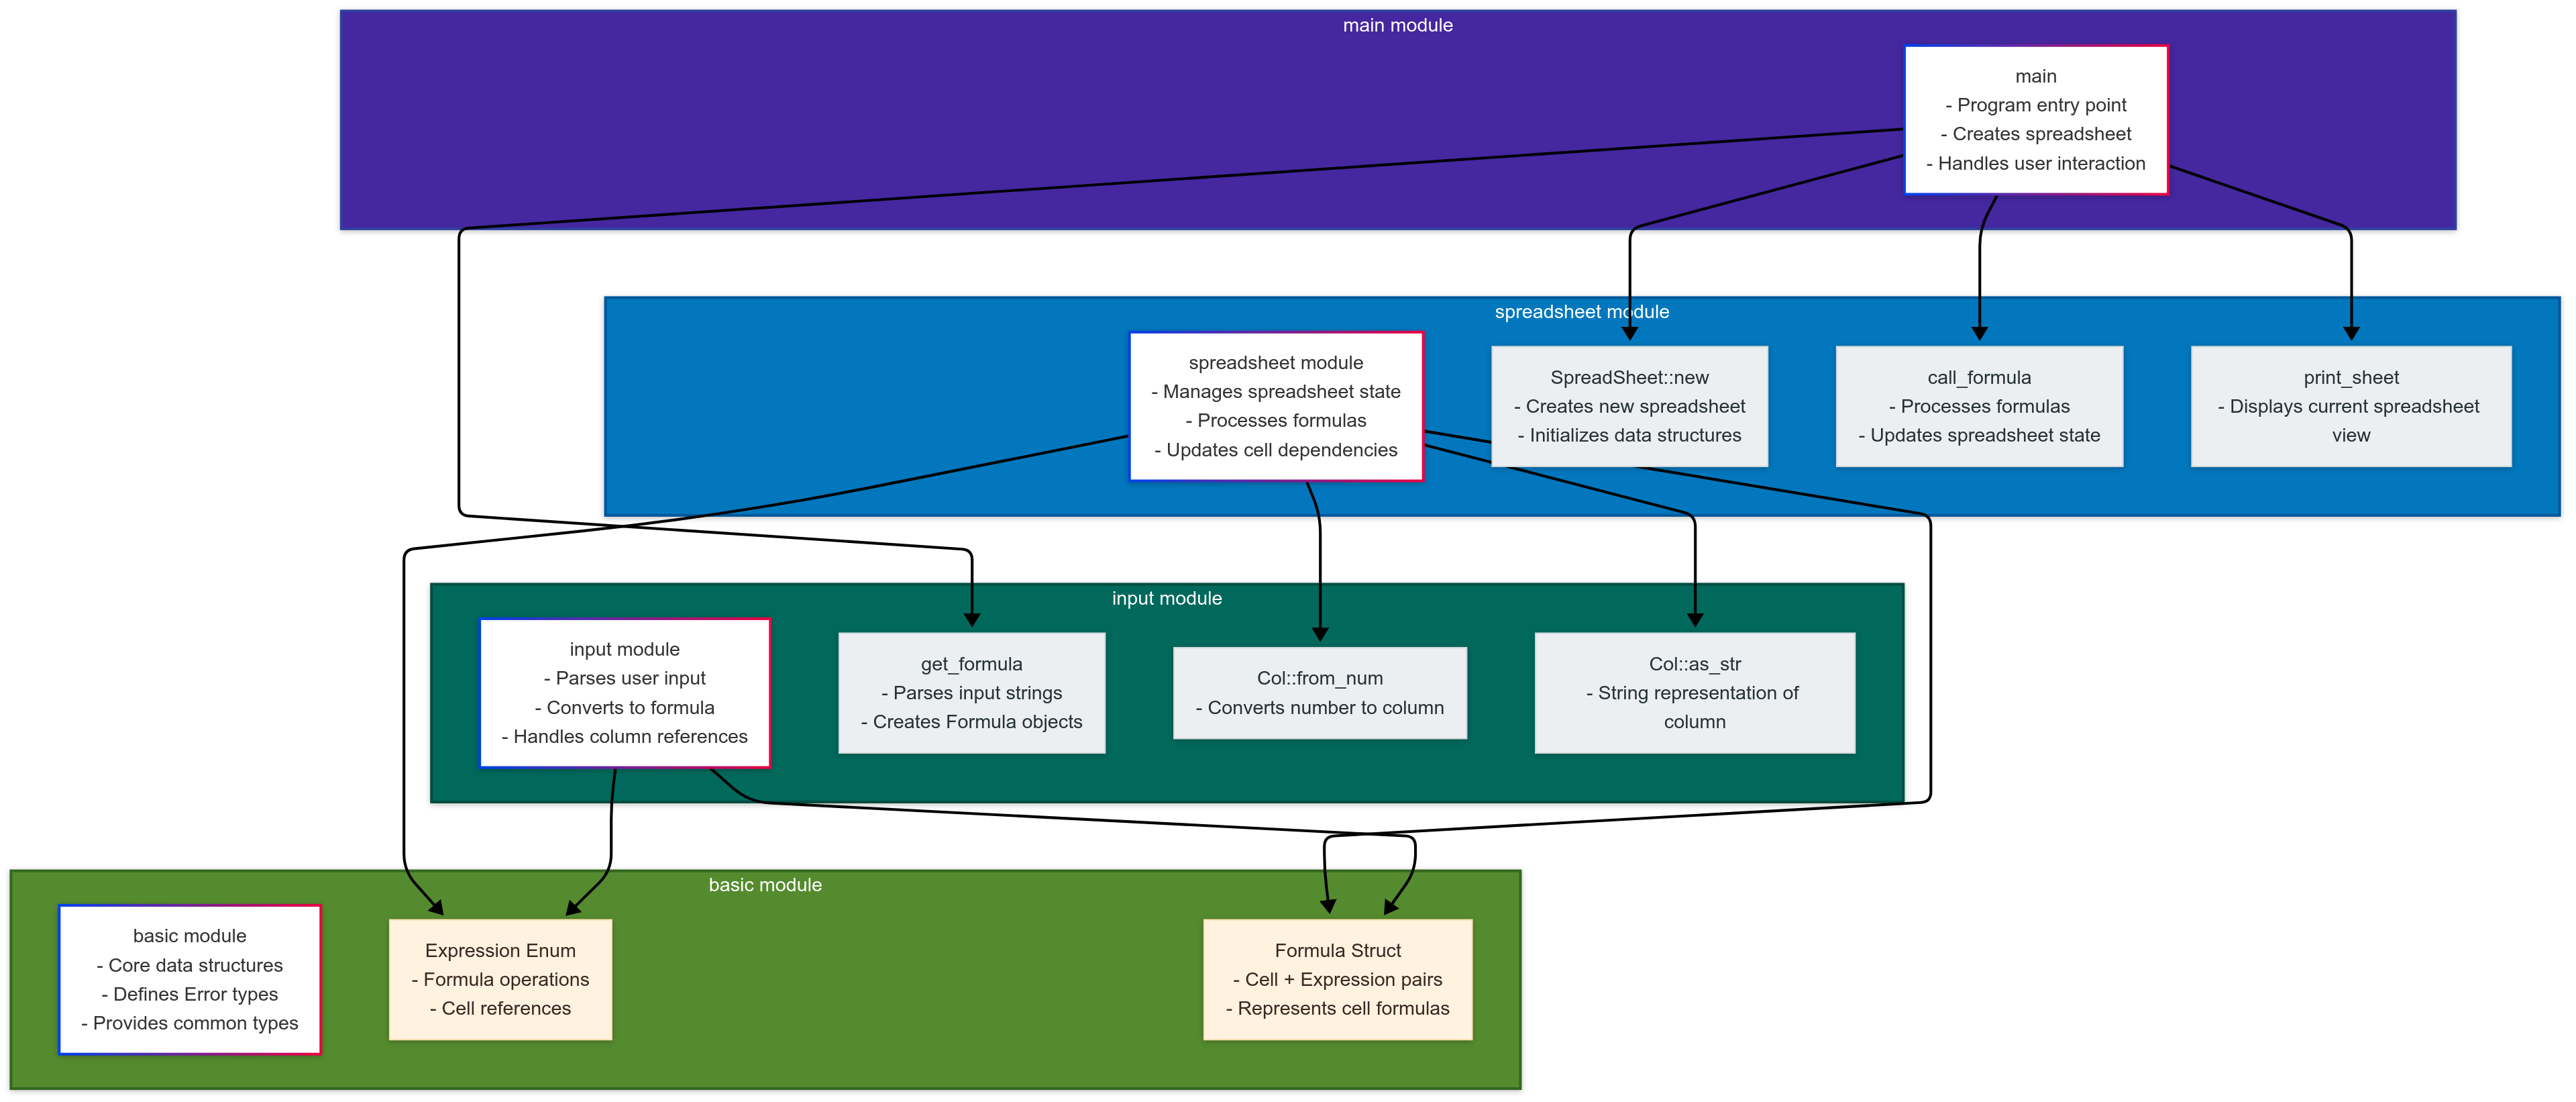
\includegraphics[width=1.1\linewidth]{Overview.png}
    \caption{Overview}
    \label{fig8}
\end{figure}


\section{\bf Frontend Architecture Overview}

We store the spreadsheet on the frontend as a HashMap to save storage space, especially when using a very large spreadsheet in which most of the values are uninitialized.

\begin{verbatim}
pub cell_values: HashMap<String, String>,

struct VisualizationState {
    visible: bool,
    data: Vec<(String, Vec<(String, f64)>)>,
    title: String, // Main title from cell A1
}
\end{verbatim}

We used the Yew framework to develop the front-end of our spreadsheet application. To provide meaningful user feedback, we implemented a toast notification system that uses a global state. This system allows asynchronous error messages—such as division by zero, reference to an undefined cell, or detection of cyclic dependencies—to be displayed as temporary pop-ups at the bottom of the interface.

\section{\bf Extensions}


\subsection{IO}

Cells can be individually selected to add expressions, or the formula can be added directly in the Enter Formula field. Enter Cell field allows users to scroll to a particular cell.

\subsection{Download and Upload}

Users can download the spreadsheet as a csv or json file and upload the csv and json files back into the webpage automatically syncing with the backend. The csv file is importable to other spreadsheet softwares such as excel and google sheets. 

\begin{figure}[H]
    \centering
    
\includegraphics[width=1\linewidth]{bar.png}
    \caption{Top Bar}
    \label{fig1}
\end{figure}

\subsection{Data Analytics}

There are two ways to view the data graphically in this spreadsheet. The analyze button will be automatically detect rows of data and graph in various formats for user convenience.

\begin{figure}[H]
    \centering
    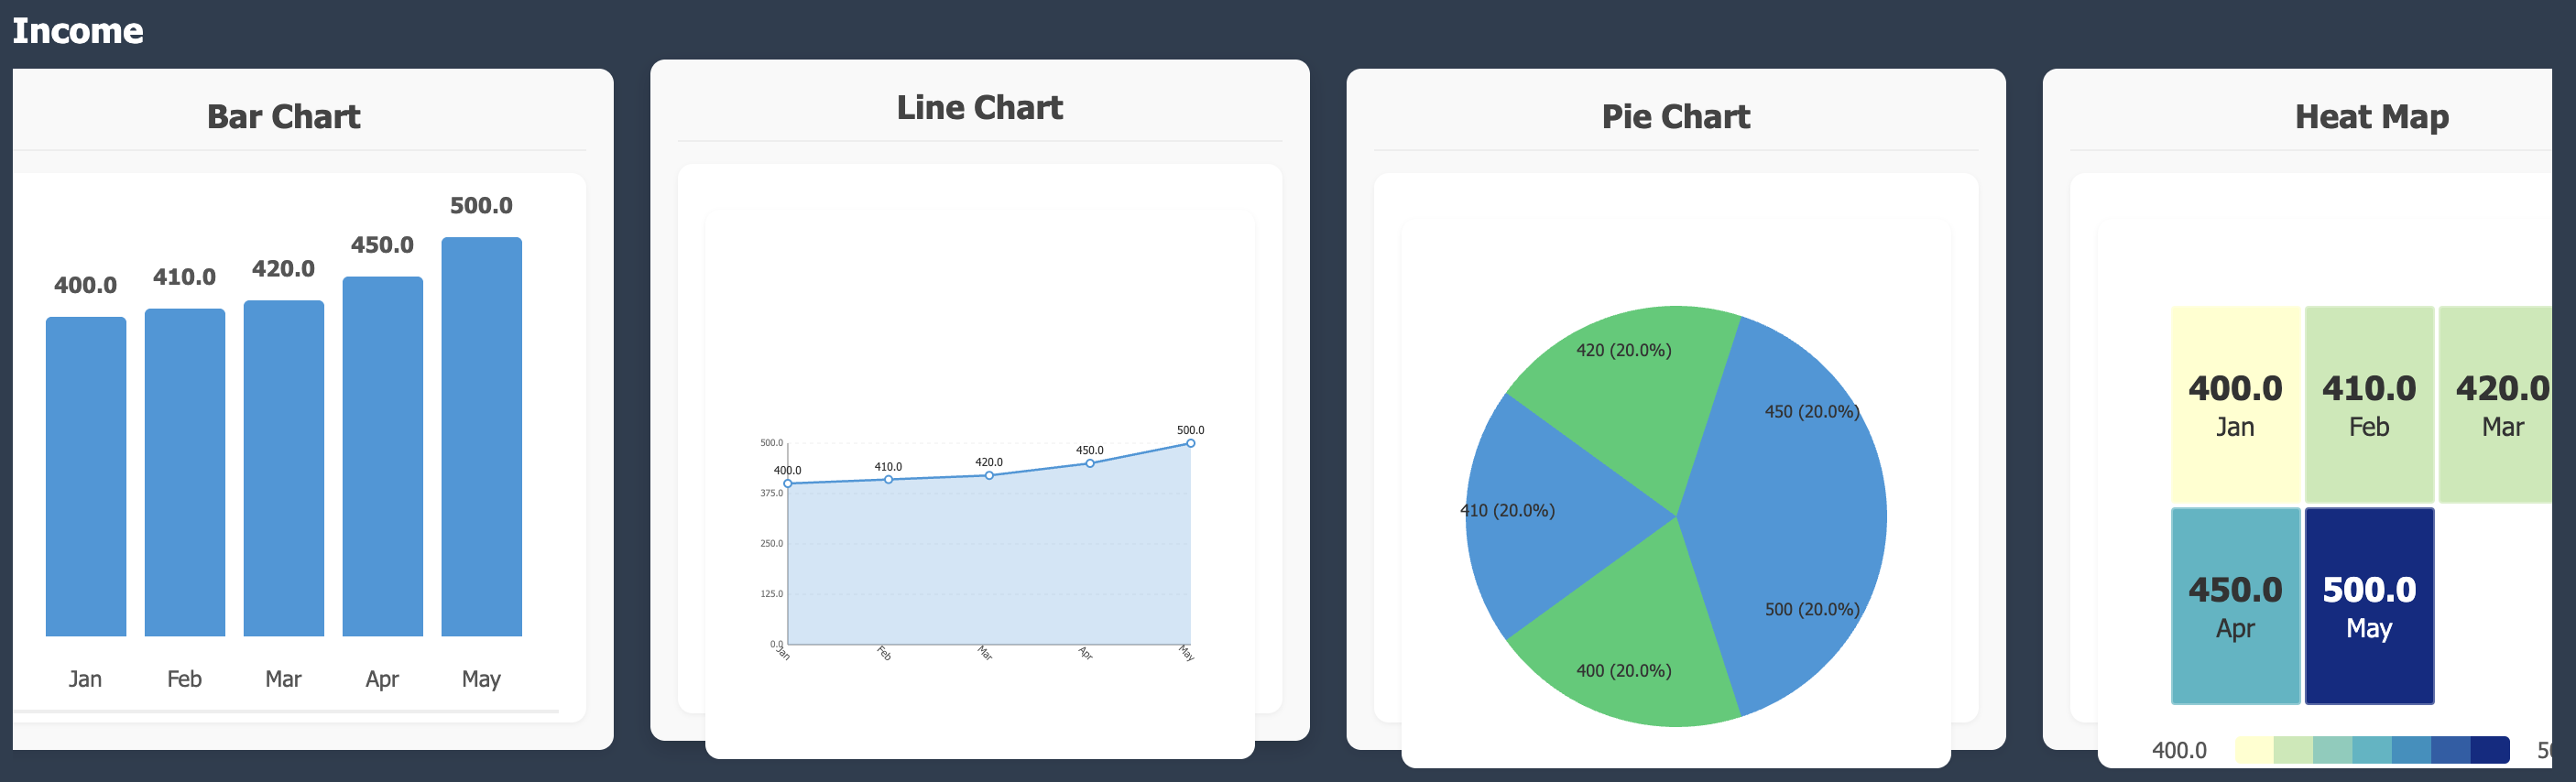
\includegraphics[width=0.5\linewidth]{analyze.png}
    \caption{Analyze Feature}
    \label{fig2}
\end{figure}

The statistics button gives a prettier overview of the data in various formats, specifically tailored for spending/budgeting spreadsheets.

\begin{figure}[H]
    \centering
    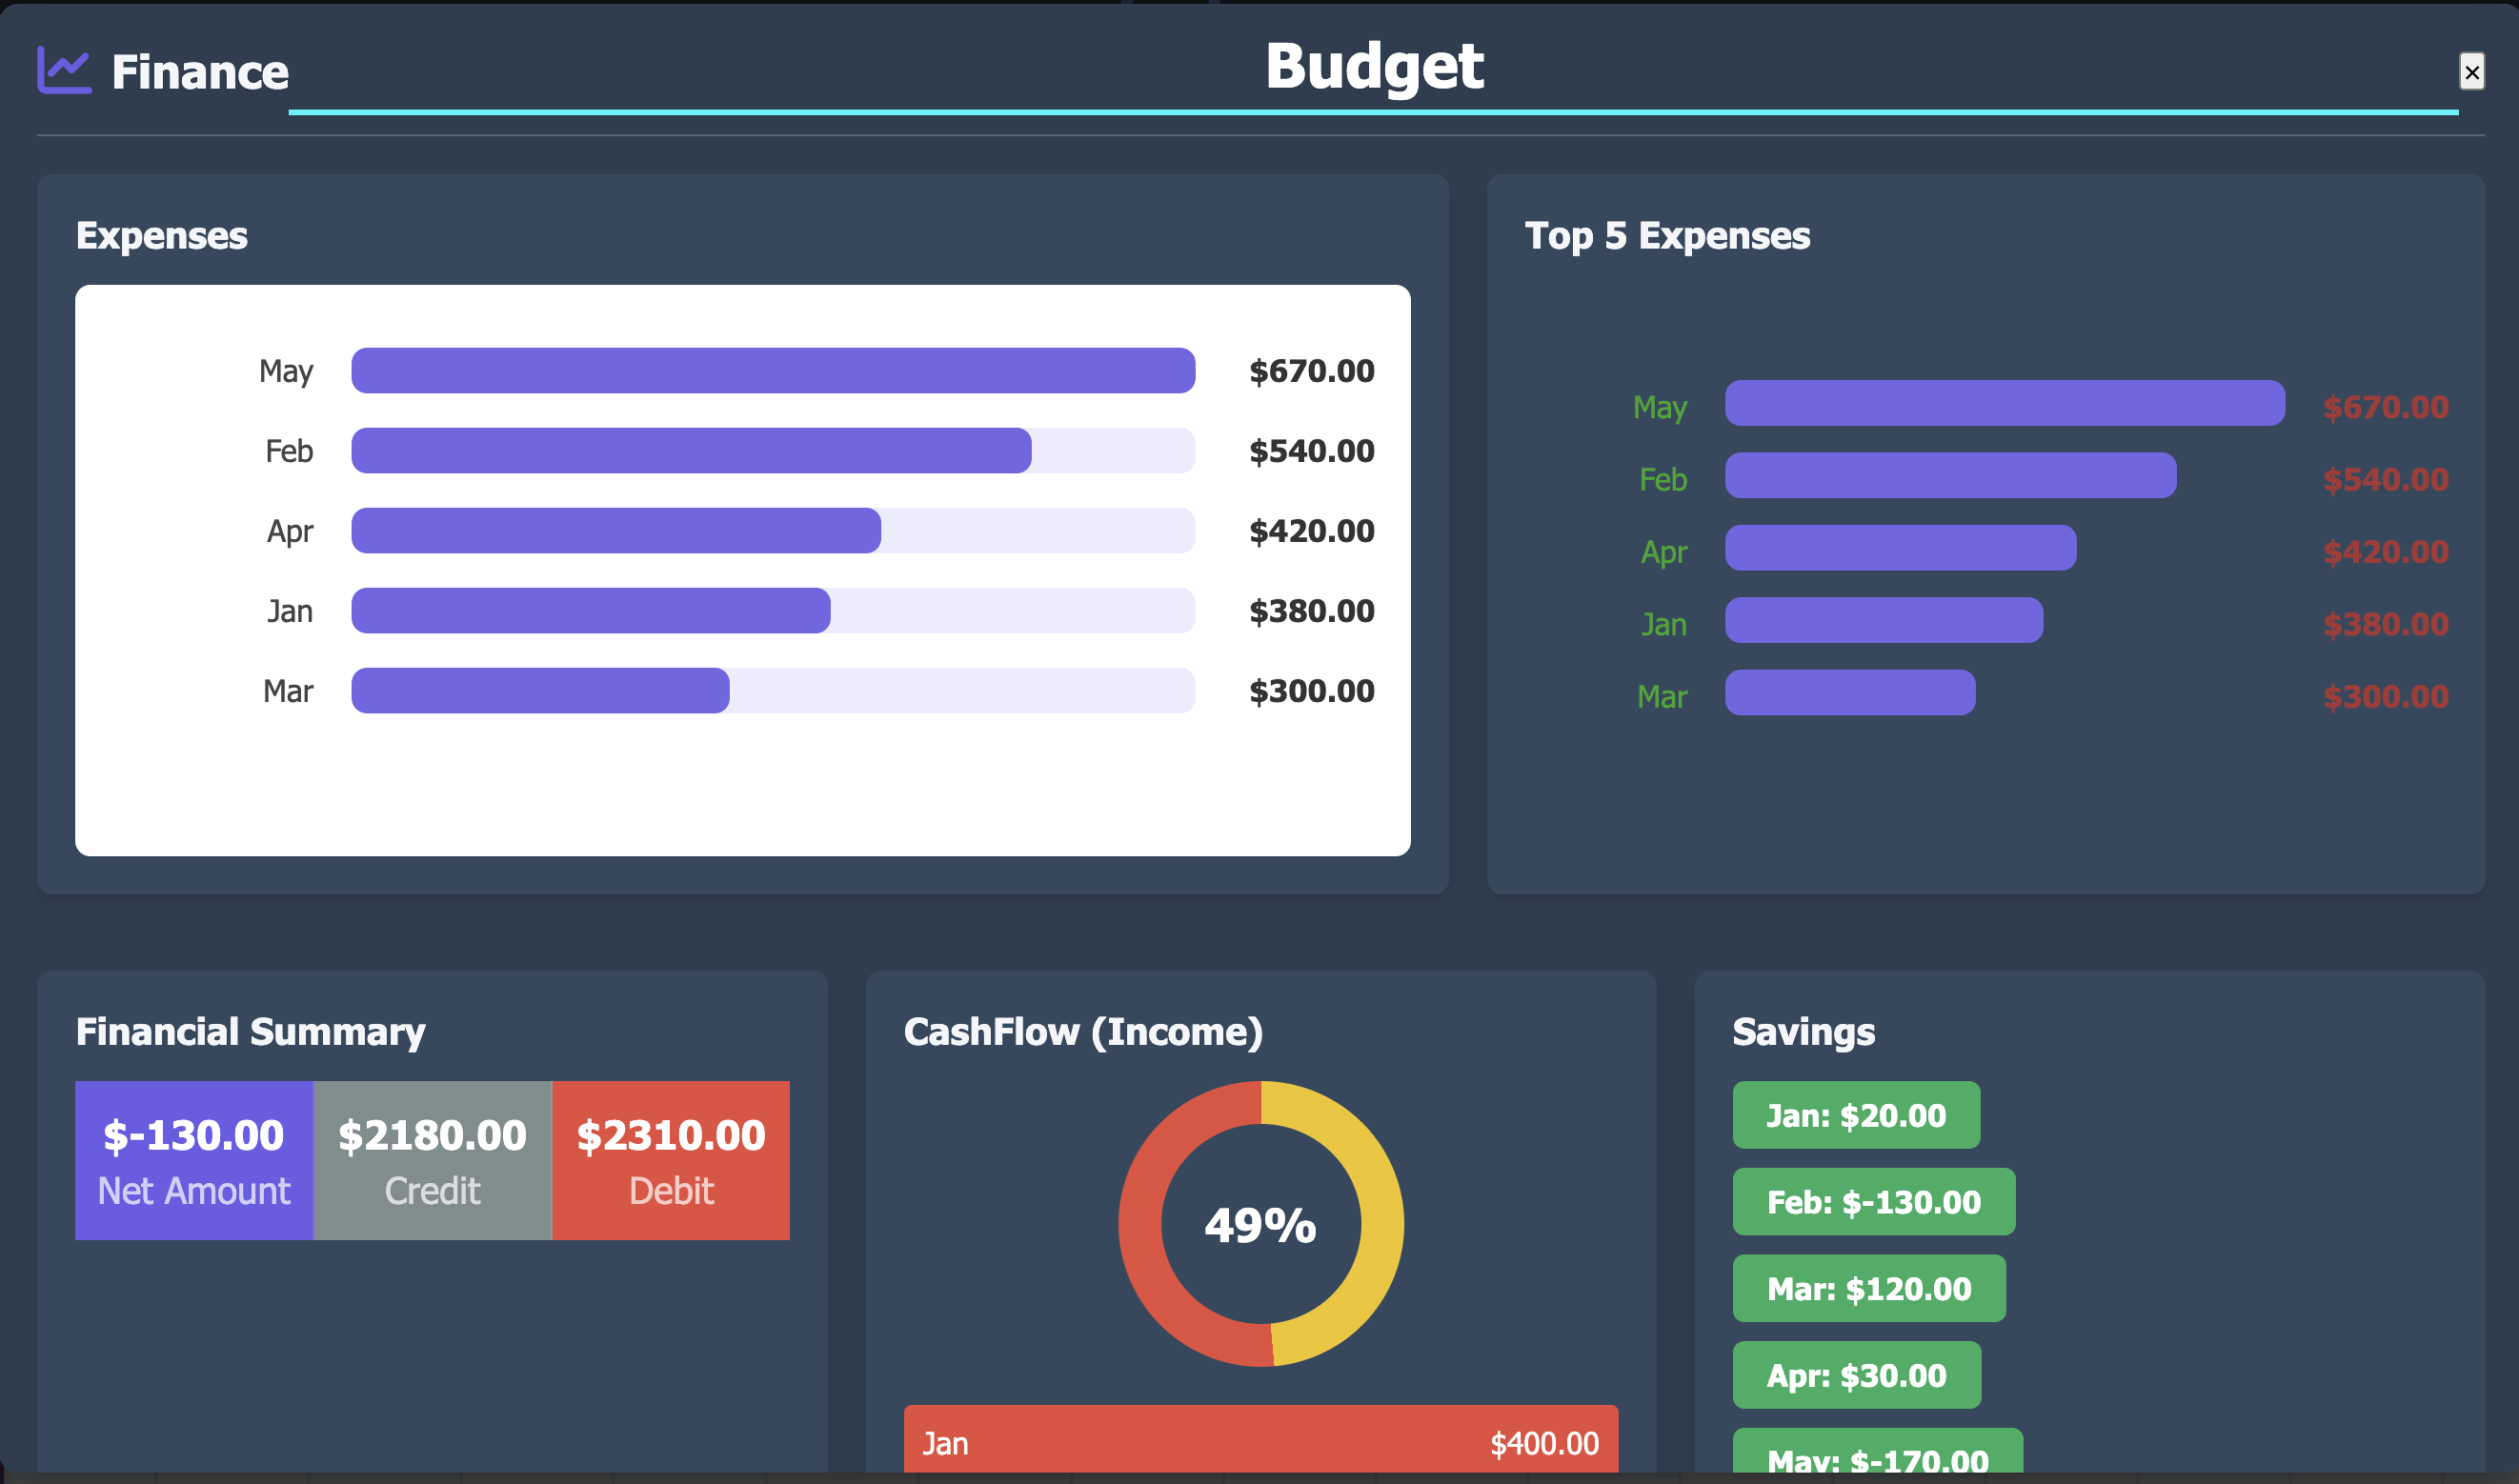
\includegraphics[width=0.5\linewidth]{statistics.png}
    \caption{Statistics Feature}
    \label{fig3}
\end{figure}

\subsection{AI Formulas}

We also allow users to prompt cohere ai to predict the next formula.
For example, I entered the following formulas in the spreadsheet, A1 = B1 + 1, A2 = B2 + 2, ..., A5 = B5 + 5. Cohere then recommended this formula.

\begin{figure}[H]
    \centering
    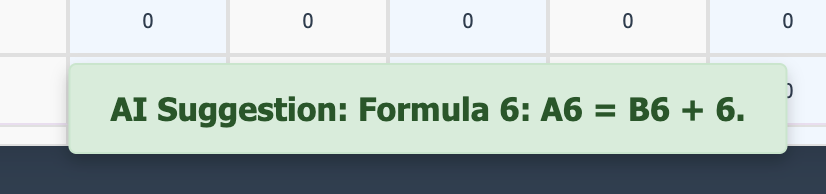
\includegraphics[width=0.75\linewidth]{cohere1.png}
    \caption{Cohere Response 1}
    \label{fig4}
\end{figure}

In another instance, I added factorial values in the spreadsheet. A1 = 1, A2 = 2, A3 = 6, A4 = 24. Here is what cohere predicted the next formula to be.

\begin{figure}[H]
    \centering
    
\includegraphics[width=0.75\linewidth]{cohere2.png}
    \caption{Cohere Response 2}
    \label{fig5}
\end{figure}

\section{Conclusion}

We were able to implement the main extensions mentioned in the proposal, creating a backend which stored the spreadsheet and a frontend server that requested the backend for spreadsheet data. We also implemented saving, graphing and ai functionality into the spreadsheet. 

Since the ai we were using was a free opensource LLM, the quality of responses was subpar, thus one of the improvements would be to use a stronger LLM. We also just used the LLM for suggesting new formulas, while in reality the usecases of AI are tremendous.

\begin{itemize}
    \item \textbf{Formula Validation:} AI can check if formulas are correctly referencing the right cells and if the operations are logical, ensuring the accuracy of calculations.
    \item \textbf{Data Consistency Checks:} AI can identify discrepancies in data, such as missing valuesm, incorrect totals, misaligned dependencies, or mismatched data types, helping to ensure data integrity.
    \item \textbf{Pattern Recognition:} AI can detect patterns in data that may be indicative of errors or outliers, helping to spot unusual data points that may require further review.
    \item \textbf{Smart Insights and Analytics:} AI can analyze the data and provide actionable insights, such as trends, correlations, or predictions, to enhance decision-making.
\end{itemize}


We encountered some issues while designing the spreadsheet. Initially we wanted the frontend to make a POST request to the backend and have the backend query the ai, and then return a response. However, there seemed to be an issue with having await statements in a function returning a POST request. Thus, we had to change the design and implement the querying from the frontend itself.

\end{document}
